%% If you prefer -- and have been allowed -- to use
%% Arial, then
%% \documentclass[arial]{usmthesis}
%% It's not really Arial, it's a Helvetica look-alike,
%% but if you're not a designer nor a typographer, you
%% probably can't tell the difference (I can't either)
\documentclass{usmthesis}
%%%%%%%%%%%%%%%%%%%%%%%%%%%%%%%%%%%%%%%%%%%%%%%%%%%%%%%
% This is usmthesis.tex, Aug 27 2015.
% Created by Lim Lian Tze (Ph.D.)
% liantze@gmail.com
% http://liantze.penguinattack.org.
%
% This is the "main" file for the thesis,
% formatted according to the Guide to the
% Preparation, Submission and Examination of
% Theses, published by IPS USM.
%%%%%%%%%%%%%%%%%%%%%%%%%%%%%%%%%%%%%%%%%%%%%%%%%%%%%%%

%% Example of loading other packages that you may require.
%% I'm loading the marvosym package so that I can produce a
%% smiley face with the command \Smiley.
\usepackage{marvosym}

%% Also, the enumitem package is great for customising
%% list environments.
\usepackage{enumitem}

%% Listings is a nice package for typesetting code
%% listings. Other possible packages include fancyvrb,
%% minted, etc.
\usepackage{listings}
\lstset{basicstyle=\ttfamily,breaklines=true}

%% For those who need to produce algorithms and pseudocode.
%% There are a number of different packages available, but
%% unfortunately they tend not to work well together!
%% I'm using algorithmicx, specifically algpseucode, here.
\usepackage{algpseudocode}
\usepackage{algorithm}

%% Enter particulars about your thesis HERE
% Your Name
\author{Lim Lian Tze}
% English title of your thesis
\title{Writing Your Thesis with LaTeX with a Very, Very, Very Long Title}
% Malay title of your thesis
\titlems{Penulisan Tesis dengan LaTeX}
% Year submitted
\submityear{2015}
% Month submitted
\submitmonth{December}
%% Choose only 1 degree type! :-)
\degreetype{Doctor of Philosphy}
% \degreetype{Master of Science}


%%%%%%%%%%%%%%%%%%%%%%%%%%%%%%%%%%%%%%%%%%%%%%%%%%%%%%%
%  You can comment out the following line if you don't have a
% "List of Own Publications"
%%%%%%%%%%%%%%%%%%%%%%%%%%%%%%%%%%%%%%%%%%%%%%%%%%%%%%%
\newcites{own}{List of Publications}

%%%%%%%%%%%%%%%%%%%%%%%%%%%%%%%%%%%%%%%%%%%%%%%%%%%%%%%
% Options for generating hyperlinks when using pdfLaTeX
%%%%%%%%%%%%%%%%%%%%%%%%%%%%%%%%%%%%%%%%%%%%%%%%%%%%%%%
\ifpdf
  \makeatletter
  \usepackage[pdftex,plainpages=false,hypertexnames=false,bookmarksnumbered,pdfpagelabels,%
    pdfauthor={\@author},pdftitle={\@title}]{hyperref}
  \makeatother
\else
  \usepackage[dvips,plainpages=false,bookmarksnumbered,breaklinks=true]{hyperref}
\fi

\usepackage{ragged2e}
\begin{document}

%%%%%%%%%%%%%%%%%%%%%%%%%%%%%%%%%%%%%%%%%%%%%%%%%%%%%%%
% Default bibliography style is apa (using 
% \RequirePackage[natbibapa]{apacite} in the class file).
%
% If you prefer the number system though, use bibliography
% style "plainnat" for [1][2][3] or "alpha" for [Jon94] (the label
% will be auto-generated).
%%%%%%%%%%%%%%%%%%%%%%%%%%%%%%%%%%%%%%%%%%%%%%%%%%%%%%%
\bibliographystyle{apacite}
\bibliographystyleown{apacite}
%\bibliographystyle{plainnat}
%\bibliographystyleown{plainnat}

\frontmatter

%%%%%%%%%%%%%%%%%%%%%%%%%%%%%%%%%%%%%%%%%%%%%%%%%%%%%%%
% Inserts the cover page (the hard cover with gold-lettering)
% and the title page 
%%%%%%%%%%%%%%%%%%%%%%%%%%%%%%%%%%%%%%%%%%%%%%%%%%%%%%%
\makecover


%%%%%%%%%%%%%%%%%%%%%%%%%%%%%%%%%%%%%%%%%%%%%%%%%%%%%%%
% MAKE SURE YOU HAVE A acknowledgements.tex FILE
%%%%%%%%%%%%%%%%%%%%%%%%%%%%%%%%%%%%%%%%%%%%%%%%%%%%%%%
\chapter{Acknowledgements}

Many thanks to Prof.~Donald Knuth for giving us \TeX, and Leslie Lamport for \LaTeX.  

I first learned \LaTeX{} as an undergraduate student in Computer Science at the University of Warwick. Back in Malaysia, I picked it up again while doing my M.Sc.~at USM, as part of some productive procrastination (there I've admitted it!!). This coincided with Dr.~Dhanesh's and Dr.~Azman's efforts in raising awareness about \LaTeX{} at USM during NaCSPC'05 -- somehow one thing led to another, and I now conduct trainings and consultatons on \LaTeX. \Smiley

Since then, many friends and fellow \LaTeX{} users have given feedback and helped relayed important updates from IPS to me, to help improve the class and template. It has actually come to a point where you are too numerous to name! Thank you all, as well as everyone who has attended my talks and workshops, used my various templates, downloaded examples from my website (\url{http://liantze.penguinattack.org/latextypesetting.html}).

Hope everyone graduates quickly then!

%Thanks to Dr.~Donald Knuth for giving us \TeX, Leslie Lamport for \LaTeX, the NaCSPC'05 committee and Dr.~Dhanesh for spreading the \LaTeX word and material.

%Hope everyone graduates quickly!

\begin{singlespace}
\tableofcontents \clearpage
\listoftables \clearpage
\listoffigures \clearpage
%%%%%%%%%%%%%%%%%%%%%%%%%%%%%%%%%%%%%%%%%%%%%%%%%%%%%%%
% You can comment out the following line if you don't
% have a "List of Plates"
%%%%%%%%%%%%%%%%%%%%%%%%%%%%%%%%%%%%%%%%%%%%%%%%%%%%%%%
\listofplates \clearpage

%%%%%%%%%%%%%%%%%%%%%%%%%%%%%%%%%%%%%%%%%%%%%%%%%%%%%%%
% You can comment out the following line if you don't
% have a "List of Acronyms"
%%%%%%%%%%%%%%%%%%%%%%%%%%%%%%%%%%%%%%%%%%%%%%%%%%%%%%%
\chapter{List of Abbreviations}

\begin{acronym}[UTMK] %% replace 'MMMM' with the longest acronym in your list
\acro{IPS}{Institut Pengajian Siswazah}
\acro{PPSK}{Pusat Pengajian Sains Komputer}
\acro{USM}{Universiti Sains Malaysia}
\acro{UTMK}{Unit Terjemahan Melalui Komputer}
\end{acronym}

\chapter{List of Symbols}

\begin{acronym}[lim ]
\acro{lim}[$\lim{}$]{limit}
\acro{theta}[$\theta{}$]{angle in radians}
\end{acronym}

\end{singlespace}

% Paragraph spacing
\setlength\parskip{18pt}
% Text-float spacing
\setlength\intextsep{24pt}

%%%%%%%%%%%%%%%%%%%%%%%%%%%%%%%%%%%%%%%%%%%%%%%%%%%%%%%
% Your Malay and English abstracts, each in one file.
%%%%%%%%%%%%%%%%%%%%%%%%%%%%%%%%%%%%%%%%%%%%%%%%%%%%%%%
\begin{MsAbstract}
Ini merupakan abstrak Melayu untuk tesis USM.  Ianya disediakan dengan sistem penyediaan dokumen \LaTeX.
\end{MsAbstract}
\begin{EnAbstract}

This is the English abstract of a USM thesis.  It was prepared with the \LaTeX\ document typesetting system.

\end{EnAbstract}

 
\mainmatter

%%%%%%%%%%%%%%%%%%%%%%%%%%%%%%%%%%%%%%%%%%%%%%%%%%%%%%%
% The actual chapters of your thesis as listed in 
% mainchaps.tex. Make sure you have the relevant
% chapter files. 
% E.g. if you mainchaps.tex contains the lines
%
%  \include{hypothesis.tex}
%  \include{proof.tex}
%
% Then you MUST have the files hypothesis.tex, proof.tex
% (containing the relevant chapters) in the same directory
% as mainchaps.tex.
%%%%%%%%%%%%%%%%%%%%%%%%%%%%%%%%%%%%%%%%%%%%%%%%%%%%%%%
\chapter{Introduction: Samples of Basic \LaTeX{} Commands}\label{chap:intro}

Hello and welcome, fellow \ac{USM} research postgrad!  The \verb|usmthesis| package and template files were written in the hope that they may help you prepare your research thesis using \LaTeX, based on the \ac{IPS} requirements \citep{ips:thesis:guideline:2007}. \textbf{Please note that this version is based on the \emph{new} guidelines, in force 17 Dec 2007 onwards.}

\LaTeX{} is powerful and produces beautiful documents.  However, there is definitely a learning curve to it -- one that is worth the effort.  %This is also a learning process for the author, so 
If you find any errors in these templates or documents, or have any suggestions or feedback, do e-mail me about it (\path{liantze@gmail.com}).  The author cannot always guarantee prompt response, however. \Smiley

MiK\TeX{}, my recommended \LaTeX{} distribution for Windows, is available on the CSPC'07 CD. A step-by-step installation walkthrough is available at \citep{lim:latextypesetting}.

\section{Some Simple Command Usages}

There are plenty of free \LaTeX{} tutorials online, some of which are listed in the bibliographies or available at \url{http://e-office.cs.usm.my}.  This sample thesis includes some examples to do some common tasks.  We start with some examples for lists (both bulleted and numbered), highlighting texts in bold and italic, and URLs:

\lstset{breaklines=true, basicstyle=\small\ttfamily, language=[LaTeX]TeX, columns=fullflexible, framesep=10pt, xleftmargin=16pt, keywordstyle={\mdseries}}

\begin{figure}[htb!]
\begin{lstlisting}
\begin{enumerate}
\item bulleted and numbered lists, 
\item footnotes\footnote{This is a footnote. However note that footnotes are not encouraged for the sciences.}, 
\item font effects such as

\begin{itemize}
\item \textbf{bold}, 
\item \emph{italic}, and 
\item \texttt{typewriter-like}
\end{itemize}

\item URLs and e-mail addresses: \url{http://www.cs.usm.my/~llt/}, \url{dummy.add@hotmail.com};
\item citations: see Chapter \ref{chap:review}.
\end{enumerate}
\end{lstlisting}
\caption{Common Layout and Formatting Tasks}\label{fig:simple}
\end{figure}

\begin{enumerate}
\item bulleted and numbered lists, 
\item footnotes\footnote{This is a footnote. However note that footnotes are not encouraged for the sciences.}, 
\item font effects such as

\begin{itemize}
\item \textbf{bold}, 
\item \emph{italic}, and 
\item \texttt{typewriter-like}
\end{itemize}

\item URLs and e-mail addresses: \url{http://www.cs.usm.my/~llt/}, \url{dummy@hotmail.com};
\item citations: see Chapter \ref{chap:review}
\end{enumerate}

Incidentally, if you feel that the lists above are too far apart vertically, use the \textbf{compactenum} and \textbf{compactitem} environments instead.  The effect is then like the following:

\begin{figure}[htb!]
\begin{lstlisting}
\begin{compactenum}
\item item one,
\item item two,
\item item three.
\end{compactenum}

\begin{compactitem}
\item item one,
\item item two,
\item item three.
\end{compactitem}
\end{lstlisting}
\caption{Compact Lists}\label{fig:paralist}
\end{figure}


\begin{compactenum}
\item item one,
\item item two,
\item item three.
\end{compactenum}

\begin{compactitem}
\item item one,
\item item two,
\item item three.
\end{compactitem}

Granted, the lists are still wide, but this is because we need to honour the requirement for double line-spacing.

\section{Special Characters}

Bear in mind that certain characters are special \LaTeX{} symbols and need to be escaped, as shown in Table~\ref{tab:special:char}.

\begin{table}[htb!]
\caption{Special Characters in \LaTeX}\label{tab:special:char}
\centering
\begin{singlespace}\begin{tabular}{|c | l | l|}
\hline
Symbol & Name & Escape code \\\hline\hline
\# & \normalsize{hash, pound} & \verb|\#| \\
\$ & \normalsize{dollar} & \verb|\$| \\
\% & \normalsize{percent} & \verb|\%| \\
\^{} & \normalsize{``hat''} & \verb|\^{}| \\
\& & \normalsize{ampersand} & \verb|\&| \\
\_ & \normalsize{underscore} & \verb|\_| \\
\{ & \normalsize{left brace} & \verb|\{| \\
\} & \normalsize{right brace} & \verb|\}| \\
\~{} & \normalsize{tilde} & \verb|\~{}| \\
$\sim$ & \normalsize{wide tilde} & \verb|$\sim$| \\
`` & \normalsize{open double quotes} & \verb|``| \\
'' & \normalsize{close double quotes} & \verb|''| \\
\hline
\end{tabular}\end{singlespace}
\end{table}

Note that for quotation marks, you might prefer \verb|``this'' and `that'|  (``this'' and `that')
instead of \verb|"this" and 'that'|  ("this" and 'that').

If you need to typeset special characters (such as \Stopsign, \Biohazard, \Smiley, $\curvearrowright$, etc), take a look at the Comprehensive \LaTeX\ Symbol List. It should be under \path|C:\Program Files\MiKTeX 2.5\doc\info\symbols\comprehensive\symbols-a4.pdf| if you installed MiKTeX on a Windows machine.


\section{Useful Resources}\label{sec:resources}
\citep{latex:companion} is a \emph{very} useful book --- but it's quite an investment at RM180++.  A worthy one, nevertheless.  \citet{roberts} has a website with very good \LaTeX{} tutorials at \url{http://www.comp.leeds.ac.uk/andyr/misc/latex/}, too.  Don't forget the famous \texttt{lshort} tutorial \citep{lshort}.

I've also compiled a list that I find useful at \url{http://liantze.googlepages.com/latextypesetting} \citep{lim:latextypesetting}, which also hosts slide materials I presented at the Introductary \LaTeX{} Workshop at CSPC'07.  % note need to use \input here for \addtocontents{toc}... to work
\chapter{Citations and Bibliography}\label{chap:review}

This chapter should have been a survey on the history of \TeX{} and \LaTeX{}, and a comparison to conventional word processors in preparing academic documents.  Due to lack of time on the author's part, and also the abundance of such discussions on the web, we look at ways to prepare the bibliography and citations instead.

\section{The \texttt{*.bib} File}
First of all, bear in mind that your bibliography file (\verb|*.bib| files) is like a database.  That means you can maintain a centralised list, and reuse it for all your publications.  \LaTeX{} will only list sources that you actually cite in the text for each document, according to the bibliography and citation style you select in each document.  But you can still hack it so that your own publications are listed, even if you did not cite it.
 

\begin{figure}[htb!]
\begin{lstlisting}[language={}]
@BOOK{latex:companion,
  title = {The \LaTeX{} Companion},
  publisher = {Addison-Wesley},
  year = {2004},
  author = {Frank Mittelbach and Michel Goosens and Johannes Braams and David Carlisle and Chris Rowley},
  series = {Addison-Wesley Series on Tools and Techniques for Computer Typesetting},
  address = {Boston, MA, USA},
  edition = {2nd}
}
\end{lstlisting}
\caption{A BibTeX Entry}\label{fig:bibtex}
\end{figure}

As an example, in \verb|mybib.bib| I created a Bib\TeX{} entry with JabRef, the source text of which is shown in Figure~\ref{fig:bibtex}.

One thing to note about authors' names: Bib\TeX{} recognises ``Mittelbach'' as the last name for both \texttt{Frank Mittelbach} and \texttt{Mittelbach, Frank}.  So for a name like ``Lim Lian Tze'', you would have to specify it as either \texttt{Lian Tze Lim} or \texttt{Lim, Lian Tze} for Bib\TeX{} to recognise ``Lim'' as the last name correctly.  In addition, if the surname or family name of an author consists of multiple words, enclose it with braces to avoid surprises, like so: \texttt{Syed Muhammad Naquib \{al-Attas\}}.

\section{Citations using the \texttt{natbib} package}
The \verb|usmthesis| package imports the \verb|natbib| package which provides flexible citation mechanisms, so see its documentation for more details.  On a MiK\TeX{} or Pro\TeX{}t installation,
% it should be in \url{texmf/doc/latex/natbib/natbib.dvi} or \url{natbib.pdf}, in the path where you installed MiKTeX. 
use the command prompt to issue \lstinline|mthelp --view natbib| to access the documentation.
On teTeX, simply type \verb|texdoc natbib| and the documentation will be displayed automatically, if it's found on your machine.

The basic citation commands are \verb|\citet| and \verb|\citep|, which stands for \emph{textual} and \emph{parenthetical} citation respectively.  They take extra arguments, too, for adding notes in the citations.  

\subsection{Author-Year System}
Author-year styles include those in the Harvard package, such as \texttt{agsm, dcu, kluwer} and others.
If you're using an author-year system, like I did for this sample thesis, you get the following:

\begin{compactitem}
\item \verb|\citet{latex:companion}| $\to$ \citet{latex:companion}
\item \verb|\citet[chap.~2]{latex:companion}| $\to$ \citet[chap.~2]{latex:companion}
\item \verb|\citep{latex:companion}| $\to$ \citep{latex:companion}
\item \verb|\citep[chap.~2]{latex:companion}| $\to$ \citep[chap.~2]{latex:companion}
\item \verb|\citep[see also][]{latex:companion}| $\to$ \citep[see also][]{latex:companion}
\item \verb|\citep[see also][chap.~2]{latex:companion}| $\to$ \citep[see also][chap.~2]{latex:companion}
\item \verb|\citet{latex:companion,roberts}| $\to$ \citet{latex:companion,roberts}
\item \verb|\citep{latex:companion,roberts}| $\to$ \citep{latex:companion,roberts}
\end{compactitem}

You may also want to write only the author's name or year occassionally:

\begin{compactitem}
\item \verb|\citeauthor{latex:companion}| $\to$ \citeauthor{latex:companion}
\item \verb|\citeyear{latex:companion}| $\to$ \citeyear{latex:companion}
\item \verb|\citeyearpar{latex:companion}| $\to$ \citeyearpar{latex:companion}\end{compactitem}

\subsection{Numeric System}

If you prefer the plain, numerical system, do the following steps first:
\begin{compactenum}
  \item In \texttt{usmthesis.cls}, search for the line \verb|\RequirePackage{natbib}| and modify it to:\\
  \verb|\RequirePackage[numbers]{natbib}|
  \item In \texttt{usmthesis.tex}:
  \begin{compactitem}
    \item comment out the line starting with \verb|\citestyle{...}|
    \item modify the \verb|biblography| styles to: \\
      \verb|\bibliographystyle{plainnat}| \\
      \verb|\bibliographystyleown{plainnat}|
    \end{compactitem}
    or any other number system style that you prefer.
\end{compactenum}

You will then get the following citation outputs: 


\begin{compactitem}
\item \verb|\citet{latex:companion}| $\to$ Mittelbach et al. [1]
\item \verb|\citet[chap.~2]{latex:companion}| $\to$ Mittelbach et al. [1, chap.~2]
\item \verb|\citep{latex:companion}| $\to$ [1]
\item \verb|\citep[chap.~2]{latex:companion}| $\to$ [1, chap.~2]
\item \verb|\citep[see also][]{latex:companion}| $\to$ [see also 1]
\item \verb|\citep[see also][chap.~2]{latex:companion}| $\to$ [see also 1, chap.~2]
\item \verb|\citet{latex:companion,roberts}| $\to$ Mittelbach et al. [1], Roberts [3]
\item \verb|\citep{latex:companion,roberts}| $\to$ [1, 3]
\item \verb|\citeauthor{latex:companion}| $\to$ Mittelbach et al.
\item \verb|\citeyear{latex:companion}| $\to$ 2004
\item \verb|\citeyearpar{latex:companion}| $\to$ [2004]
\end{compactitem}

\chapter{Figures, Tables, Equations, Algorithms, etc}\label{chap:design}

%Your design chapter.  I probably should include some examples on inserting figures, tables, mathematical equations, etc.

(This is supposed to be the design or methodology chapter.  Instead, we include examples on inserting figures, tables, mathematical equations\ldots i.e.\ things that you might want to include in your thesis.)

\section{Inserting Figures}\label{sec:figure}

%When using \LaTeX{}, you can't exactly draw figures on-the-fly as you do in WYSIWYG word processors like Word.  (Well, actually you CAN, but the \LaTeX{} way of line drawings is still beyond this author.)  
You can draw diagrams with special \LaTeX\ commands, but this may take some extra time to learn.  I've had some forays into the \texttt{pgf} and \texttt{tikz} packages and must say I quite like the results; but as I said, they take time to learn. If you want a faster solution, you can draw your diagrams using other applications, and saving them as graphic files (EPS, PNG, JPG, PDF).  

\LaTeX{} requires EPS (encapsulated postscript) graphic files when generating DVI output, and PNG, JPG or PDF when generating PDF output.  (I have never got GIF files to work.  If you have, please let me know.)

%I myself create the diagrams in Powerpoint (since sooner or later I'll have to give some sort of presentation about my project anyway), saving them as PNG, and then export the PNG files.

For exporting to EPS, I use GIMP, the open-source (and free-of-charge) equivalent of Photoshop\footnote{GIMP runs on Windows too, but remember to install GTK2+ first.  You'll find the download links on the GIMP website at \url{http://www.gimp.org/}.  If you're comfortable with the command line interface, you may consider ImageMagick, too.}.  I see an export to EPS option too in Photoshop, but the resultant file just doesn't seem to work with \LaTeX.

Do note that IPS \textbf{discourages} the use of colours in your thesis, including diagrams and figures.  Phographs and colour plates are exceptions to this rule: see Section~\ref{sec:plate}.

Here's how to insert a picture with the filename \verb|pythag.eps| or \verb|pythag.png|.  I'm going to display it here with 5cm width, and the caption ``Pythagoras' Theorem''.

\begin{figure}[hbtf!]
\begin{lstlisting}
\begin{figure}[hbtf!]\centering
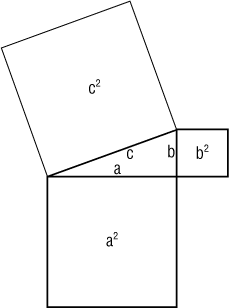
\includegraphics[width=50mm]{pythag}
\caption{Pythagoras' Theorem}\label{fig:pythagoras}
\end{figure}
\end{lstlisting}
\caption{Including a Graphics File}\label{fig:lst:graphics}
\end{figure}

The result would be:

\begin{figure}[hbtf!]\centering
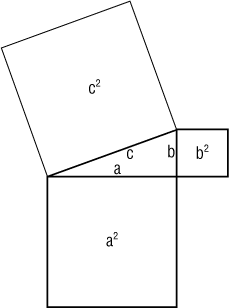
\includegraphics[width=50mm]{pythag}
\caption{Pythagoras' Theroem} \label{fig:pythagoras}
\end{figure}

Don't specify the extension of the graphic file.  The template will automatically look for the EPS or the PNG (or otherwise) versions, depending on whether \verb|latex| or \verb|pdflatex| was used.  The \texttt{figure} environment will also ensure that that an entry is inserted into the \emph{List of Figures} automatically -- including the figure numbering, caption and page number.

In addition, the width of the included graphics can also be specified as a percentage of the text width, e.g.~ \verb|width=.2\textwidth| would cause the graphics to occupy 20\% of the text width.

Notice that I inserted a \verb|\label| just after the \verb|\caption|.  This can be used for referencing the figure number, like this: \\
\verb|Figure \ref{fig:pythagoras}| $\to$ Figure \ref{fig:pythagoras}

This works the same for chapters, sections, tables, equations too.  In \verb|chap-intro.tex|, I labelled the Introduction chapter with \verb|\label{chap:intro}|.  I also labelled the section on inserting figures, \verb|\label{sec:figure}|.  So now I can do \\
\verb|Chapter \ref{chap:intro}| $\to$  Chapter \ref{chap:intro} \\
\verb|section \ref{sec:figure}| $\to$  section \ref{sec:figure}

Everytime the numbering of the heading changes, the reference will change automatically as well.  \textbf{This is another advantage of using \LaTeX{}}: you do not need to manually update the reference counters (nor the Table of Contents, List of Figures and Tables) whenever you add or remove figures, tables, sections or chapters.

You might also want to try out \texttt{JpgfDraw}: it is a vector graphics and drawing application (requiring Java), and can export to \LaTeX{} code which you can paste into your \LaTeX{} source. \texttt{JpgfDraw} is available from \url{http://theoval.cmp.uea.ac.uk/~nlct/jpgfdraw/index.html}.


\section{Inserting Plates}\label{sec:plate}

Colour photographs are now regarded as \emph{plates}. They must be listed in the \emph{List of Plates} instead of the List of Figures, and should be printed in colour on glossy photo paper \citep{ips:thesis:guideline:2007}.

The \texttt{usmthesis} document class defines a new \texttt{plate} environment, as well as a corresponding \verb|\listofplates| command.  (The \verb|\listofplates| command is already placed in the sample template file \verb|usmthesis.tex|.)  In short, all you need to do to insert a photograph or plate (as a graphics file \verb|USMScience.{eps,png,jpg}|) is shown in Figure~\ref{fig:lst:plate}, and you will then get Plate~\ref{plate:ppsk:usm} as the result.


\begin{figure}[hbtf!]
\begin{lstlisting}
\begin{plate}[hbtf!]\centering
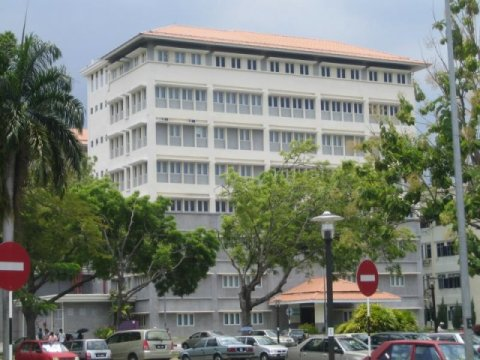
\includegraphics[width=.9\textwidth]{USMScience}
\caption{School of Computer Sciences, USM}\label{plate:ppsk:usm}
\end{plate}
\end{lstlisting}
\caption{Inserting a Plate}\label{fig:lst:plate}
\end{figure}

\begin{plate}[hbtf!]\centering
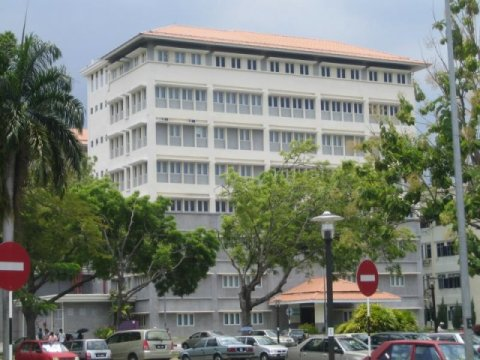
\includegraphics[width=.9\textwidth]{USMScience}
\caption{School of Computer Sciences, USM}\label{plate:ppsk:usm}
\end{plate}


\section{Inserting Tables}

Typesetting tables can be a little troublesome especially with complex layouts.  Look up \citep{roberts} to learn about some tips, or you can use the \textrm{LaTable} program (\url{http://www.g32.org/latable/}) to help you.

If using \textrm{LaTable}, when you're done designing the table, copy the whole table as \LaTeX\ code, and paste it in your source file.  (You may add additional formatting commands, like bold, italics, etc.)  If this is going to be a numbered table, remember to surround it with \verb|\begin{table}| and \verb|\end{table}|, and give it a caption, like this:

\begin{figure}[hbtf!]
\begin{lstlisting}
\begin{table}[hbtf!]\centering
\begin{tabular}{| l | c || r |}
\hline
\textbf{Name} & \textbf{Category} & \textbf{Quantity} \\ 
\hline\hline
Apple & Fruit & 10 \\ 
\hline
Cucumber & Vegetable & 25 \\ 
\hline
Daisy & Flower & 5 \\ 
\hline
\end{tabular}
\caption{Sample Table Only} \label{table:sample}
\end{table}
\end{lstlisting}
\caption{Typesetting Tables}\label{fig:lst:table}
\end{figure}

\begin{table}[hbtf!]\centering
\begin{tabular}{| l | c || r |}
\hline
\textbf{Name} & \textbf{Category} & \textbf{Quantity} \\ 
\hline\hline
Apple & Fruit & 10 \\ 
\hline
Cucumber & Vegetable & 25 \\ 
\hline
Daisy & Flower & 5 \\ 
\hline
\end{tabular}
\caption{Sample Table Only} \label{table:sample}
\end{table}

Note also that \verb|usmthesis| is configured such that captions for figures are placed \emph{below} the figures, and captions for tables are placed \emph{above} them, in accordance with the formatting guidelines.

%Many of us would have had massive headaches about lining up decimal places in table columns (as mentioned in the IPS guidelines) if not for this tip from \citep[pp.~274--276]{latex:companion}. This method uses the \verb|dcolumn| package (already loaded by \verb|usmthesis.cls|). Instead of using \verb|l,c| or \verb|r| as the column type in the \verb|tabular| declaration, use\\ \texttt{D\{\textit{input sep}\}\{\textit{output sep}\}\{\textit{decimal places}\}}.
%
%\begin{figure}[htb!]
%\begin{lstlisting}
%\begin{table}[htb!]\centering
%\begin{tabular}{| c | D{.}{.}{2} |}
%\hline
%Item & \multicolumn{1}{c|}{Reading}\\\hline
%A & 1.11\\\hline
%B & 3.99\\\hline
%C & 2.27\\\hline
%\end{tabular}
%\caption{A table with decimal data}
%\end{table}
%\end{lstlisting}
%\caption{Aligning decimal data in tables}\label{fig:align:decimal}
%\end{figure}
%
%The \LaTeX\ code in Figure~\ref{fig:align:decimal} will give you Table~\ref{tab:align:decimal}.
%
%\begin{table}[htb!]\centering
%\begin{tabular}{| c | D{.}{.}{2} |}
%\hline
%Item & \multicolumn{1}{c|}{Reading}\\\hline
%A & 1.11\\\hline
%B & 3.99\\\hline
%C & 2.27\\\hline
%\end{tabular}
%\caption{A table with decimal data}\label{tab:align:decimal}
%\end{table}
%
%Without using \verb|dcolumn|, you'd get something like this:
%
%\begin{table}[htb!]\centering
%\begin{tabular}{| c | r |}
%\hline
%Item & \multicolumn{1}{c|}{Reading}\\\hline
%A & 1.111\\\hline
%B & 3.999\\\hline
%C & 2.277\\\hline
%\end{tabular}
%\caption{A table with decimal data (mis-aligned)}
%\end{table}


\section{Full-paged, Sideways Figures and Tables}

To make a figure appear on a landscape, full-page layout, put your \verb|\includegraphics| command in a \verb|sidewaysfigure| environment (Figure~\ref{fig:lst:sidewayfigure}).

\begin{figure}[htb!]
\begin{lstlisting}
\begin{sidewaysfigure}\centering
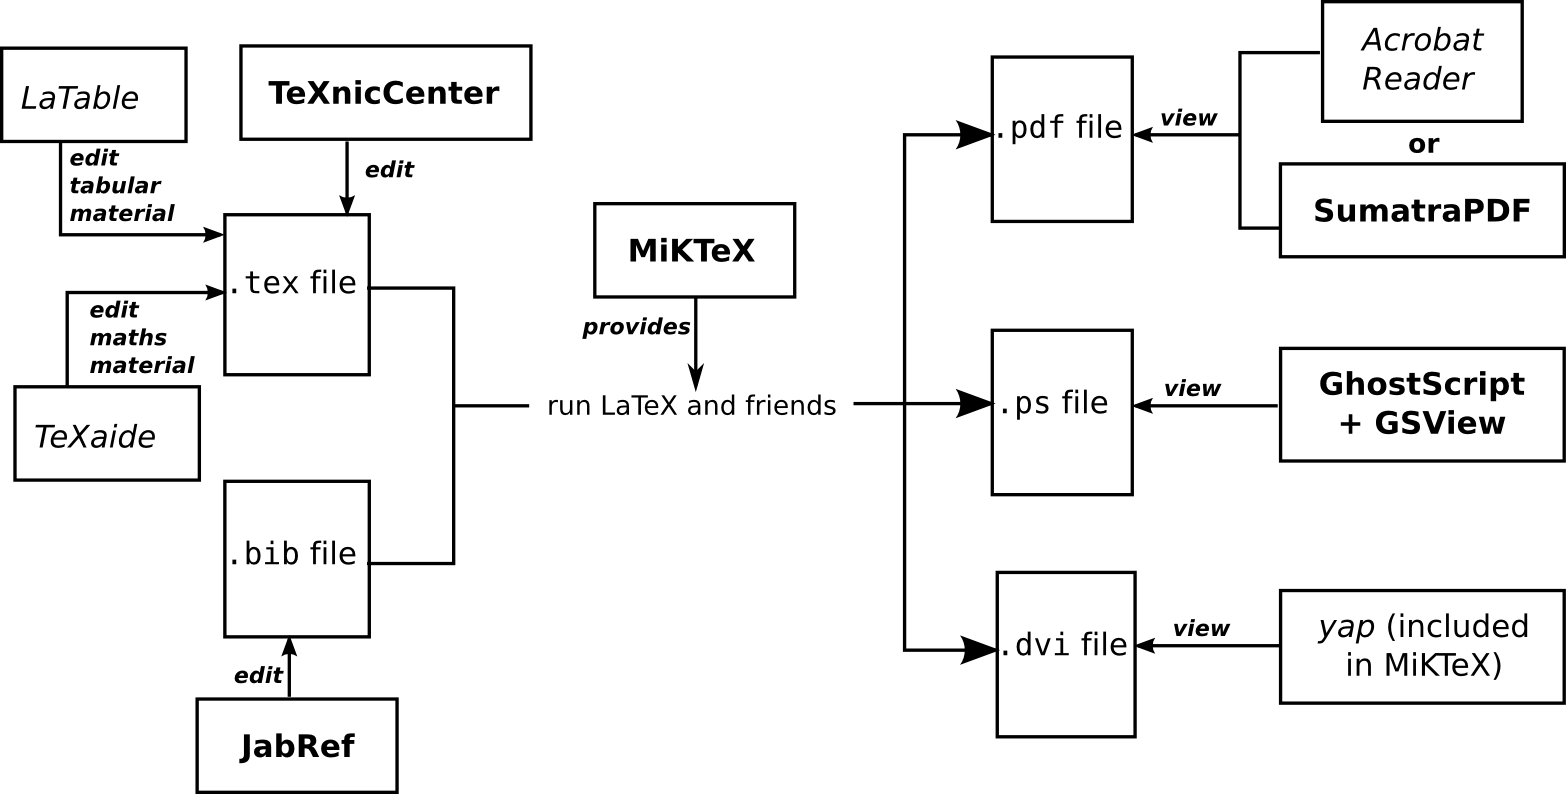
\includegraphics[width=\textheight]{latex-win-comp}
\caption{A full-page, sideways figure}\label{fig:sidewaysfig}
\end{sidewaysfigure}
\end{lstlisting}
\caption{Including a sideway, full-page graphic}\label{fig:lst:sidewayfigure}
\end{figure}

\begin{sidewaysfigure}
\centering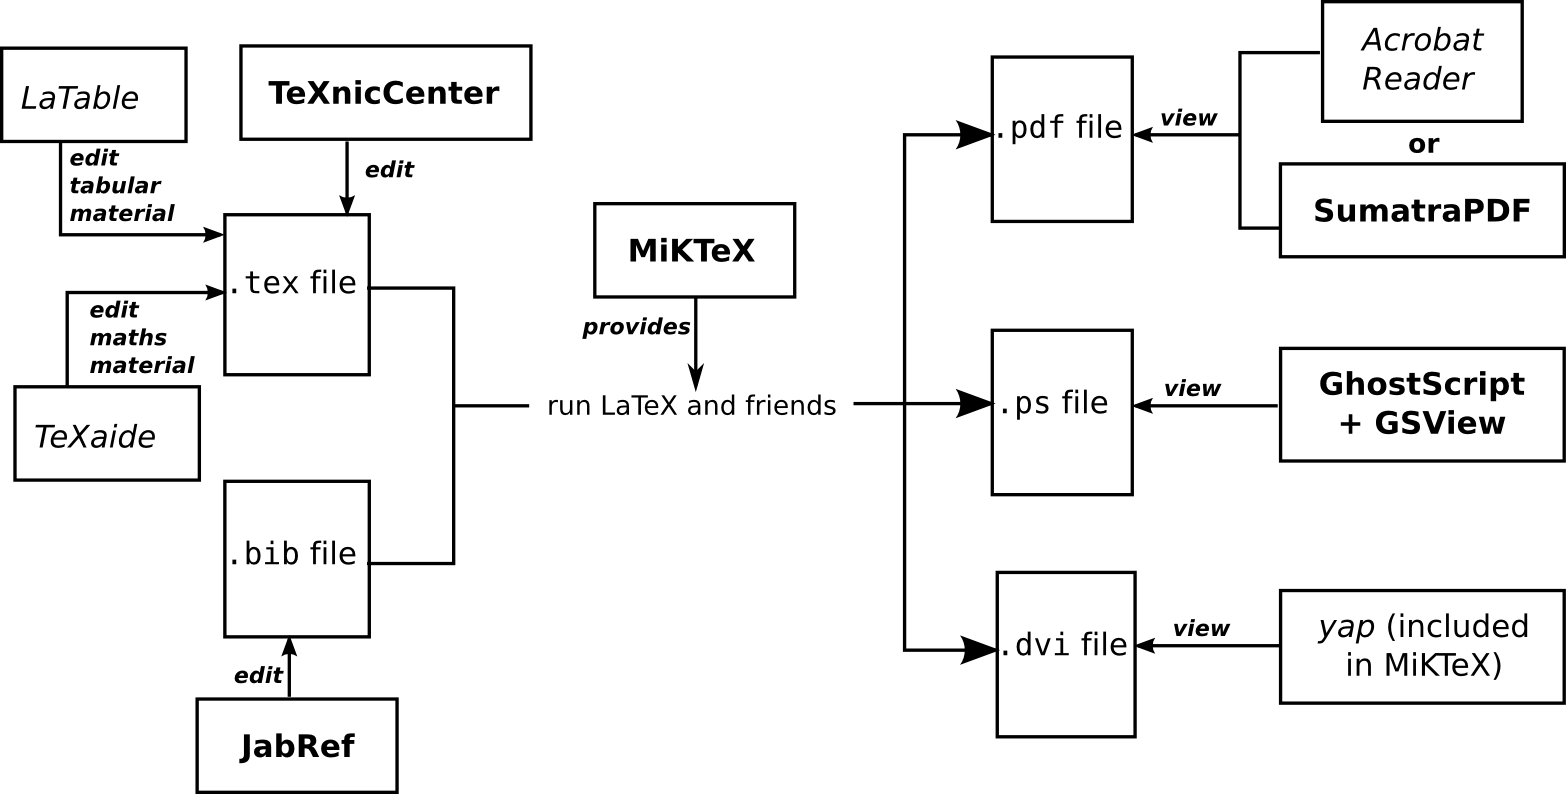
\includegraphics[width=\textheight]{latex-win-comp}
\caption{A full-page, sideways figure}\label{fig:sidewaysfig}
\end{sidewaysfigure}

The resultant figure (Figure~\ref{fig:sidewaysfig}) should appear on the next page.

For a sideways table, use the \verb|sidewaystable| environment instead around your usual \verb|tabular| material.


\section{Mathematical Equations}

%Oooh I love this one.  After all, maths is the reason why Donald Knuth created \TeX{}!  It would be quite impossible for me to list all the commands, so I'll just give some example here, and you're better off looking at the various online tutorials like \cite{roberts}.  And TeXnicCenter certainly makes things much easier.

Typesetting mathematical material is one of, if not \emph{the}, strongest capabilities of \LaTeX.  After all, that was the Knuth's main motivation for creating \TeX{}.  As it is impossible to enumerate all possible mathematically-related commands and macros here, we will just give some examples.  The reader is directed to the many well-written online tutorials, such as \citep{roberts}, for more elaborate examples.  TeXnicCenter also provides many shortcut buttons for inserting mathematical symbols.

\begin{figure}[htb!]
\begin{lstlisting}
\begin{equation}\label{eq:pythagoras}
z^2 = x^2 + y^2
\end{equation}

\begin{equation}\label{eq:golden:ratio}
\phi = \frac{1}{2} (1 + \sqrt{5})
\end{equation}

\begin{equation}\label{eq:golden:ratio}
\phi = \frac{1}{2} (1 + \sqrt{5})
\end{equation}
\begin{equation}\label{eq:golden:ratio:fibonacci}
\phi = 1 + \sum ^ {\infty} _ {n=1}
                \frac{ (-1) ^ {n+1} }{ F_n F_{n+1} }
\end{equation}

Equation~\ref{eq:pythagoras} is the Pythagoras Theorem. 
\eqref{eq:golden:ratio} gives the golden ratio $\phi$, and 
\eqref{eq:golden:ratio:fibonacci} relates it to the Fibonacci 
series.
\end{lstlisting}
\caption{Typesetting Mathematical Equations}\label{fig:lst:equation}
\end{figure}

\begin{equation}\label{eq:pythagoras}
z^2 = x^2 + y^2
\end{equation}
\begin{equation}\label{eq:golden:ratio}
\phi = \frac{1}{2} (1 + \sqrt{5})
\end{equation}
\begin{equation}\label{eq:golden:ratio:fibonacci}
\phi = 1 + \sum ^ {\infty} _ {n=1}
                \frac{ (-1) ^ {n+1} }{ F_n F_{n+1} }
\end{equation}

Equation~\ref{eq:pythagoras} is the Pythagoras Theorem. \eqref{eq:golden:ratio} gives the golden ratio $\phi$, and \eqref{eq:golden:ratio:fibonacci} relates it to the Fibonacci series.

The \LaTeX\ code to generate the above mathematics materials are shown in Figure~\ref{fig:lst:equation}.  As you can see, references to equations can be achieved with either \verb|\ref| or \verb|\eqref|. 

A disclaimer: if you think the mathematic equations don't look as great as all those \LaTeX\ advocates make them out to be, that's because IPS requires Times to be used and the current offerings of free \LaTeX\ math fonts for Times don't look great. It would've been a different picture if we used Computer Modern.

\section{Acronyms}
\acresetall
If you have a list of acronyms or symbols, edit the file \verb|loa.tex| as in Figure~\ref{fig:acronym}.

\begin{figure}[hbt!]
\begin{lstlisting}
\begin{acronym}[UTMK] %% replace 'UTMK' with the longest acronym in your list
\acro{IPS}{Institut Pengajian Siswazah}
\acro{PPSK}{Pusat Pengajian Sains Komputer}
\acro{USM}{Universiti Sains Malaysia}
\acro{UTMK}{Unit Terjemahan Melalui Komputer}
\end{acronym}
\end{lstlisting}
\caption{The template \texttt{loa.tex} for acronyms}\label{fig:acronym}
\end{figure}

You can also use this acronym list to help expand it the first time you mention it in your text.  For example, the first time you use \verb|\ac{USM}|, `\ac{USM}' will be the output (without the quotes).  After that, all calls to \verb|\ac{USM}| will give `\ac{USM}' (without the quotes).  For more information, see the documentation for the \texttt{acronym} package.


\section{Typesetting Algorithms}

As computer scientists, it is quite common to include algorithms.  The \verb|algorithmic| package is very handy for this.  Its documentation, found under the \verb|doc/latex/algorithms| subdirectory of the \LaTeX\ installation directory, is very helpful.  We reproduce a short example from the documentation here.

\begin{figure}[hbt!]
\begin{lstlisting}
\begin{algorithmic}
\REQUIRE $n \geq 0$
\ENSURE $y = x^n$
\STATE $y \Leftarrow 1$
\STATE $X \Leftarrow x$
\STATE $N \Leftarrow n$
\WHILE{$N \neq 0$}
\IF{$N$ is even}
\STATE $X \Leftarrow X \times X$
\STATE $N \Leftarrow N / 2$
\ELSE[$N$ is odd]
\STATE $y \Leftarrow y \times X$
\STATE $N \Leftarrow N - 1$
\ENDIF
\ENDWHILE
\end{algorithmic}
\end{lstlisting}
\caption{Typesetting Algorithms}\label{fig:lst:algo}
\end{figure}

\begin{figure}[hbt!]
\begin{algorithmic}
\REQUIRE $n \geq 0$
\ENSURE $y = x^n$
\STATE $y \Leftarrow 1$
\STATE $X \Leftarrow x$
\STATE $N \Leftarrow n$
\WHILE{$N \neq 0$}
\IF{$N$ is even}
\STATE $X \Leftarrow X \times X$
\STATE $N \Leftarrow N / 2$
\ELSE[$N$ is odd]
\STATE $y \Leftarrow y \times X$
\STATE $N \Leftarrow N - 1$
\ENDIF
\ENDWHILE
\end{algorithmic}
\caption{Computing $x^n, n > 0$}
\end{figure}

\section{Program Listings}

You may have noticed that I used the \verb|lstlisting| environment to typeset some of the \LaTeX{} examples -- with pretty-printing\footnote{Whether you agree that it \emph{is} pretty is another story altogether.}, too, including automatic line-breaking.  For more information, see the documentation for the \verb|listings| package: it's in the \verb|doc/latex/listings| subdirectory of your \LaTeX\ installation directory.

Just to give some simple example here.  For example, to typeset a ``Hello World'' Java program with syntax highlighting, you can use the following code:

\begin{figure}[hbt!]
\begin{lstlisting}[escapechar=:,language={}]
\lstset{basicstyle=\small\ttfamily, language=Java, breaklines=true, columns=fullflexible, tabsize=2}
\begin{lstlisting}
public class HelloWorld {
	public static void main( String arg[] ) {
        for (int i = 0; i < 10; i++) {
			System.out.println( "Hello World!" + i);
		}
	}
}
\end:\{:lstlisting:\}:
\end{lstlisting}
\caption{Typesetting a Java program listing}\label{fig:lst:syntax}
\end{figure}

\lstset{keywordstyle={\bfseries}}
\begin{figure}[hbt!]
\lstset{basicstyle=\small\ttfamily, language=Java, breaklines=true, columns=fullflexible, framesep=10pt, xleftmargin=16pt, tabsize=2}
\begin{lstlisting}
public class HelloWorld {
	public static void main( String arg[] ) {
        for (int i = 0; i < 10; i++) {
			System.out.println( "Hello World!" + i);
		}
	}
}
\end{lstlisting}
\caption{A pretty-printed Java program listing with syntax highlighting}
\end{figure}


If you want to turn off the syntax highlighting, set \verb|language={}|.  (See the \verb|listings| documentation for a list of programming languages for which syntax highlighting is supported.)  You can also change the \verb|basicstyle| value to get different effects: e.g. a different font family, size or text formatting.

Here's another example for a C program:

\begin{figure}[hbt!]
\begin{lstlisting}[escapechar={:}, texcl=false,language={}]
\lstset{basicstyle=\sffamily, language=C, breaklines=true, columns=fullflexible, tabsize=2}
\begin{lstlisting}
int main() {
	int c = 0;
	c = c + 1;
	printf( "%d", c );
	return 0;
}
\end:\{:lstlisting:\}:
\end{lstlisting}
\caption{Typesetting a C program listing}\label{fig:lst:c}
\end{figure}

\begin{figure}[hbt!]
\lstset{basicstyle=\sffamily, language=C, breaklines=true, columns=fullflexible, framesep=10pt, xleftmargin=.4\textwidth, tabsize=4}
\begin{lstlisting}
int main() {
	int c = 0;
	c = c + 1;
	printf( "%d", c );
	return 0;
}
\end{lstlisting}
\caption{A pretty-printed C program listing with syntax highlighting}
\end{figure}


And here is the same C program listing \emph{without} syntax highlighting (by setting \verb|language={}|):

\begin{figure}[hbt!]

\lstset{basicstyle=\sffamily, language={}, breaklines=true, columns=fullflexible, framesep=10pt, xleftmargin=.4\textwidth, tabsize=4}
\begin{lstlisting}
int main() {
	int c = 0;
	c = c + 1;
	printf( "%d", c );
	return 0;
}
\end{lstlisting}
\caption{A C program listing without syntax highlighting}
\end{figure}

\chapter{Implementation}\label{chap:implementation}

Now is the time to ``implement'' your thesis with \LaTeX.  Go forth and typeset! Happy \LaTeX{}ing! \Smiley

\section{Printing Your Thesis}
This is \emph{very} important. Assuming you're printing your thesis from Acrobat Reader, make sure the following settings are chosen correctly in the Print window:

\begin{itemize}[nosep]
\item A4 paper size is selected.
\item Make sure your Printer settings is using A4 too.
\item No page scaling.
\end{itemize}

Otherwise, the margins of your printed outputs may go horribly wrong. Print one or two pages first to make sure everything looks fine before printing your entire thesis.
\chapter{Discussion}

Just a placeholder for the discussion chapter.
\chapter{Conclusion}

T-that's all folks.  Have fun with \LaTeX!

%%%%%%%%%%%%%%%%%%%%%%%%%%%%%%%%%%%%%%%%%%%%%%%%%%%%%%%
% The bibliography.
% You can create mybib.bib with JabRef, the program included
% in the Colloquium05 CD-ROM.  Or download from
% http://jabref.sourceforge.net/
%%%%%%%%%%%%%%%%%%%%%%%%%%%%%%%%%%%%%%%%%%%%%%%%%%%%%%%
\titlespacing*{\chapter}{0pt}{25mm}{\baselineskip}
\bibliography{mybib}


%%%%%%%%%%%%%%%%%%%%%%%%%%%%%%%%%%%%%%%%%%%%%%%%%%%%%%%
% The appendices.
% If you don't have any, you may delete everything below,
% until and including \chapter{Data Used}

Put some test data here.
\chapter{UML Diagrams}

Yet another dummy placeholder for appendix material..
%%%%%%%%%%%%%%%%%%%%%%%%%%%%%%%%%%%%%%%%%%%%%%%%%%%%%%%
\titlespacing*{\chapter}{0pt}{*-4.5}{*4}
\appendix
\chapter{Data Used}

Put some test data here.
\chapter{UML Diagrams}

Yet another dummy placeholder for appendix material.

%%%%%%%%%%%%%%%%%%%%%%%%%%%%%%%%%%%%%%%%%%%%%%%%%%%%%%%
% The list of own publications.  If you don't have one, you may
% comment out the next 4 lines.
%%%%%%%%%%%%%%%%%%%%%%%%%%%%%%%%%%%%%%%%%%%%%%%%%%%%%%%
\nociteown{lim:2007,lim:latextypesetting}
\begin{singlespace}
\bibliographyown{mybib}
\end{singlespace}

\end{document}
